\chapter{Overview}\label{ch:overview}
\section{Introduction}
The problem of missing data exists almost everywhere in the field of biology, medicine, wireless sensor networks, recommendations systems. Missing data may have different sources such as equipment malfunctions, refusal of respondents to answer certain questions, node failures, environmental conditions, depending on the application fields.
\\
Imputation is a term that denotes a procedure to replace the missing values in a data set by some plausible values. 
\\
There are many ways to approach missing data.  The following are some of the common naive approaches:
\begin{itemize}
\item Ignoring missing value
\item Mean Substitution: Replace with mean of observed available values
\item Median Substitution: Replace with median of observed available values
\item Hot deck: Technique used mostly in survey which involves filling in missing data on variables of interest from nonrespondents (or recipients) using observed values from respondents (i.e. donors) within the same survey data, with similar variable values set.
\item Cold deck:  Same as hot deck except that the data is found in a previously conducted similar survey or from other similar datasets.
\item Regression: Define a model that is estimated to predict observed values of a variable based on other variables. The model is then used to impute values in cases where that specific variable is missing. Here the available information for complete observations is used to predict the values of the missing observations
\item Linear interpolation: The last valid value before the missing value and the first valid value after the missing value are used for the interpolation. If the first or last case in the series has a missing value, the missing value is not replaced.
\end{itemize}

\noindent  All of these methods are not perfectly able to extract the complex structure, inter-relationship among variables of the data. On the other hand, neural network or particularly Deep Autoencoders are very good in finding the complex structure, correlation in the data. It will help in finding better imputation results.  
Further in most of the literatures, the missing value patterns are explained as falling into these categories \cite{little_missing_pattern}: Missing completely at random (MCAR), Missing at random (MAR), Not missing at random (NMAR).
\\
But there exists other type of missing values also which are not mentioned in most of the existing literatures : block of missing values. For example in wireless sensor data, a sensor node is unable to measure its readings for certain interval of time. So most of the existing methods, algorithms that are based on above type of missing pattern doesn't work in our case. The missing pattern is shown in Fig. \ref{fig:missing_pattern}. Here large dataset of $n$ dimensions, and values $m$. For some portion of dataset, $d_3$ to $d_n$ variables values are missing while for other dataset $d_1$ to $d_3$ variables are missing.
\begin{figure}[H]
\centering
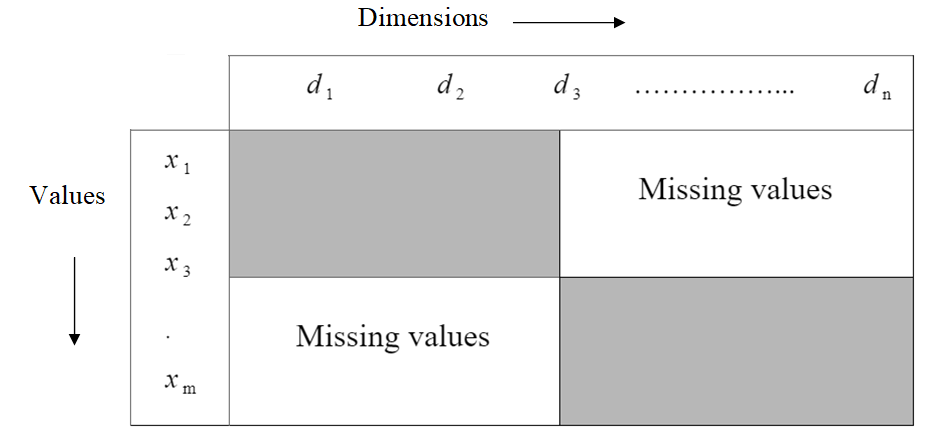
\includegraphics[width=10cm,height=5cm]{figures/missing_pattern.png}
\caption{\label{fig:missing_pattern} Missing data pattern  }
\end{figure}
\noindent
In practical cases, it is always unknown which data columns or dimensions will be missing. It actually depends on use cases. For example, if we have $10$ number of wireless sensors placed in a city and sensor number $9$ and $10$ are OFF for around $2$ hrs, then $9^{th}$ and $10^{th}$ column values will be missing up to $2$ hrs. After that, say sensor number $1$ and $2$ are OFF for another $2$ hours, $1^{st}$ and $2^{nd}$ columns will be missing. This scenario results in diagram shown in Fig \ref{fig:missing_pattern}.  
\\
In this thesis, it is proposed to solve such problem of block of missing value by using Deep Autoencoder model. As it is impossible to exactly say which columns will be missing in real world cases, it will be assumed of missing certain blocks of values and try to impute those block of missing data.
\section{Problem Definition}

Most of the machine learning algorithms, statistical conclusions are derived on based on the assumption that the dataset is complete. So, the conclusions, inferences, decisions made from incomplete dataset will have significantly negative effect. Research suggests that applications in various professional fields such as in medicine, manufacturing, energy, recommendation systems that rely on data for decision making processes may fail and lead to incorrect outcomes due to the presence of missing data. Ignoring such missing values may lead to biasness, misguide, misinformation to the readers, researchers. So it is very important to have a good method of imputation as a pre-step of any data analysis, research activities. 
\section{Objective}
\begin{itemize}
\item Impute block of missing values using deep autoencoder
\item Performance comparison between the proposed algorithm and existing state of art algorithms for imputation like mean, median
\item Validate our proposed model using Absolute Mean Error between true and imputed data
\end{itemize}
\section{Scope of the work}
The proposed thesis work will develop an imputation model that can be used in several areas where missing values exist. 
Potential use cases include:
\begin{itemize}
\item Wirless sensor networks: Data loss reasons may include depletion of a sensor's limited energy supplies, unreliable nature of wireless communications, implementation of duty cycling protocols, sparse deployment.  
\item Collaborative filtering in recommendation systems : Not all the users may provide rating. So the cold start problem can be solved with our proposed method.
\item  Economics, sociology, and political science related research because governments choose not to, or fail to, report critical statistics, researcher error for example, when data collection is done improperly or mistakes are made in data entry.
\item DNA microarrays 
\end{itemize}


